\documentclass[man]{apa7}

\input{includes/preamble_common}
\input{includes/preamble_apa7}

\title{UrbanTracker - Sistema de Georreferenciación de rutas de transporte publico}
\shorttitle{Investigación aplicada en IS}
\authorsnames{Carlos Javier Rodriguez Manchola, Jesus Ariel González Bonilla}
\authorsaffiliations{Afiliación/Institución}
\authornote{ORCID Carlos Javier Rodriguez Manchola: 0009-0005-2035-6260. Correspondencia: cjrodriguez801@soy.sena.edu.co}

\abstract{Introducción:
Se presenta UrbanTracker, un sistema de geolocalización en tiempo real diseñado para optimizar el transporte público urbano mediante el seguimiento continuo de autobuses y la gestión digital de rutas, vehículos y conductores. El proyecto surge ante la falta de información precisa para usuarios y administradores y la necesidad de soluciones asequibles adaptadas a contextos con recursos limitados (p. ej., ciudades intermedias). La validación inicial se realizó en Neiva (Colombia), pero la arquitectura propuesta es transferible a otras ciudades. La motivación se alinea con experiencias previas donde la información en vivo mejora la percepción de puntualidad y la toma de decisiones (“CITY-RUTA”, 2018; “STOPBUS”, 2016).

Métodos:
Se desarrolló una plataforma compuesta por: (i) una app móvil para conductores (GPS del smartphone), (ii) una web pública para usuarios y (iii) un panel web administrativo. El backend sigue una arquitectura hexagonal y modular con separación en domain, application e infrastructure: el modelo de dominio concentra las reglas del negocio; los servicios de aplicación orquestan los casos de uso mediante puertos/contratos; y los adaptadores de infraestructura exponen REST, manejan JPA/PostgreSQL, y conectan con mensajería en tiempo real. Los servicios REST están documentados con OpenAPI/Swagger (EasyRest, 2022), y PostgreSQL gestiona el almacenamiento relacional de rutas, vehículos, usuarios y recorridos.
Para el tiempo real se usó un flujo en el que el móvil del conductor publica posiciones por MQTT hacia un broker; el backend recibe esos mensajes, los valida y guarda, y luego envía actualizaciones por WebSockets a los clientes web (“SisMo”, 2016). La seguridad se maneja con JWT. En la interfaz, la visualización del movimiento en el mapa se implementó con Mapbox en modo 3D.
Para pruebas, se ejecutó un piloto con 1 ruta y 1 vehículo, simulando envíos periódicos de coordenadas cada ~5 s desde el móvil y suscribiendo 5–10 clientes web a las actualizaciones en vivo.

Resultados:
UrbanTracker permite visualizar en el mapa (Mapbox 3D) la ubicación de los autobuses en servicio con una frecuencia de actualización de ~5 segundos, superando un umbral mínimo de 10 s usado como referencia. La latencia medida entre el envío desde el móvil del conductor y la visualización en la web fue < 2 segundos bajo condiciones 4G normales. Se cubren las funcionalidades clave: consulta de rutas, vista de vehículos en tiempo real, inicio/cierre de recorrido por conductores y administración de rutas y flotas desde el panel. En la prueba con 5–10 suscriptores concurrentes, la solución mostró buen comportamiento, en línea con reportes previos del uso de MQTT en rastreo vehicular (“SisMo”, 2016).

Discusión:
La solución cumple lo esperado en el piloto y confirma que es viable brindar información actualizada a pasajeros y herramientas operativas a administradores con infraestructura asequible (smartphones + protocolos ligeros). La arquitectura hexagonal ayuda a separar la captura por MQTT y la difusión por WebSockets, manteniendo responsabilidades claras y facilidades para escalar. Se discuten implicaciones de seguridad y privacidad (uso de JWT y manejo responsable de datos de ubicación) y la compatibilidad con arquitecturas híbridas si crece el histórico de eventos (“Aspectos de ingeniería…”, 2022). La experiencia del usuario fue positiva: el mapa 3D facilita entender dónde está el bus y el panel simplifica tareas de gestión.

Conclusiones:
UrbanTracker evidencia que es factible mejorar la experiencia del transporte público local mediante geolocalización en tiempo real con un stack accesible. Los resultados sugieren impacto potencial en la reducción de tiempos de espera y en la eficiencia operativa. Trabajos futuros incluyen integrar más fuentes de datos en tiempo real, refinar la interfaz y ampliar las evaluaciones de usabilidad a mayor escala, manteniendo la portabilidad del enfoque a otras ciudades.}

\keywords{geolocalización, transporte público, Spring Boot, React Native, MQTT, WebSockets, JWT}

\begin{document}
\maketitle

\section{Introducción}
La incertidumbre del pasajero—no saber por dónde va el bus o cuánto falta—se reduce al mostrar posiciones en vivo, algo reportado en el transporte urbano por \cite{cityruta2018new} y \cite{stopbus2016new}. UrbanTracker busca eso y, además, facilitar la operación diaria con un panel para rutas, vehículos y conductores.

Para evitar costos de entrada altos, aprovechamos el teléfono del conductor como emisor de GPS cuando el bus no trae equipo dedicado; este enfoque ya ha sido útil en rastreo y seguridad vehicular con mensajería ligera MQTT \cite{stopbus2016new}; \cite{sismo2016}. En paralelo, una API REST clara y documentada evita malentendidos y acelera integraciones \cite{easyrest2022}; \cite{ingenieria2022}.

En móviles escogimos React Native por experiencia del equipo, aunque Flutter es una alternativa sólida de alto rendimiento en UI; conviene evaluarla cuando el proyecto crece o cambian los requisitos \cite{flutter2022new}.
\section{Marco teórico y trabajos relacionados}
Sistemas de información para transporte. Distintos proyectos han mostrado beneficios de publicar posiciones en tiempo real y permitir que el pasajero visualice rutas y buses activos \cite{cityruta2018new}; \cite{stopbus2016new}. Estas experiencias resaltan mejoras en la percepción del servicio y en la planificación del viaje.

Mensajería ligera y pub/sub. En contextos móviles y de IoT, usar MQTT con un broker como Mosquitto permite distribuir eventos con baja sobrecarga y buena escalabilidad. Trabajos de seguridad y rastreo vehicular evidencian que el patrón publish/subscribe es adecuado para manejar muchas actualizaciones de ubicación \cite{sismo2016}. Esta idea también se usa en módulos de comunicación genéricos para aplicaciones conectadas y en soluciones académicas/industriales.

APIs claras y mantenibilidad. Documentar el contrato de la API (OpenAPI/Swagger) reduce ambigüedades y acelera la integración \cite{easyrest2022}. La literatura sobre diseño orientado a objetos y sostenibilidad del software pone énfasis en separar responsabilidades y favorecer la extensibilidad \cite{poo2023}.

Arquitecturas híbridas y datos. Decidir cuándo usar almacenamiento relacional y cuándo incorporar componentes NoSQL es clave al escalar servicios de rastreo. Guías sobre sistemas híbridos ayudan a elegir la mezcla adecuada según el tipo de consulta y el volumen de eventos \cite{ingenieria2022}.

Escalabilidad en la práctica. Migraciones exitosas de monolitos a microservicios en sistemas de transporte (como el caso Kbus) reportan millones de registros diarios y cientos de miles de consultas, lo que prueba que estos dominios pueden crecer mucho \cite{torres2020}. En logística, soluciones cloud de tracking confirman el valor de ver el momento exacto de los movimientos y notificar a usuarios clave \cite{odesanya2025}. También hay experiencias recientes de rastreo en tiempo real en contextos con infraestructura desafiante \cite{anyango2025}.

Síntesis y vacíos. En conjunto, la literatura respalda: (i) publicar datos en vivo; (ii) usar canales ligeros (MQTT/WebSockets); (iii) documentar APIs; y (iv) diseñar para escalar. Persisten vacíos en guías paso a paso que integren todas estas piezas para contextos locales con presupuesto limitado. UrbanTracker llena parte de ese espacio con una receta técnica concreta y validaciones iniciales.
\section{Metodología de investigación aplicada}
\subsection{Diseño}
Se empleó un diseño de investigación-acción con ciclos planificar–actuar–observar–reflexionar, complementado con estudio de caso sobre el desarrollo y la puesta en marcha de UrbanTracker. Se fijaron principios (simplicidad, bajo costo, escalabilidad), criterios de éxito (actualización en ~5 s y latencia <2 s del móvil a la web, panel usable) y un plan de evaluación que combinó verificaciones funcionales y mediciones extremo a extremo.

\subsection{Comparación de metodologías ágiles}
Para seleccionar prácticas ágiles se realizó una evaluación multi-criterio (claridad de roles, cadencia, facilidad de adopción, riesgo). El resultado inclinó la balanza hacia Scrum (iteraciones cortas, roles definidos) con prácticas de Kanban (flujo visual y límites de WIP) para el trabajo operativo continuo.

\begin{figure}[htbp]
    \centering
    % 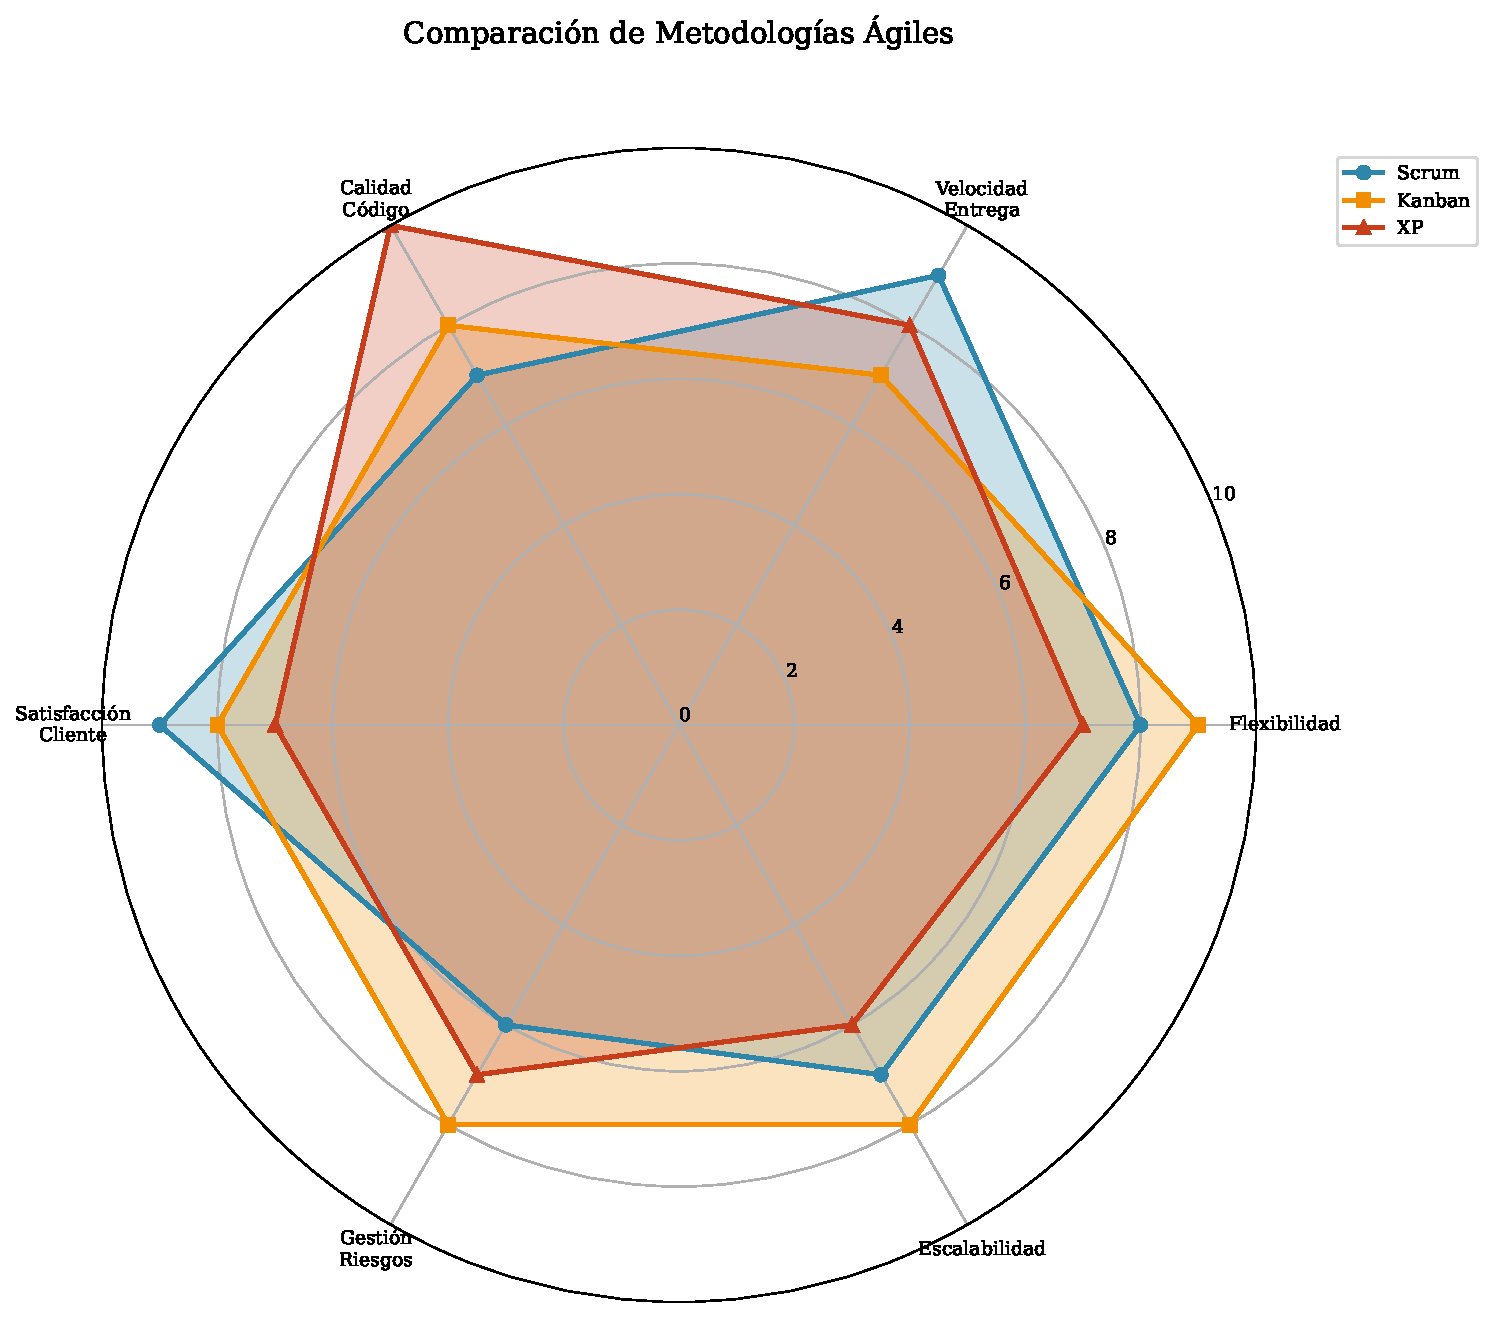
\includegraphics[width=0.45\textwidth]{graphics/comparacion_metodologias.pdf} % Inserta aquí tu gráfico cuando lo tengas
    \caption{Comparación multi-criterio de metodologías ágiles: Scrum, Kanban y XP}
    \label{fig:comparacion_metodologias}
\end{figure}

\subsection{Datos e instrumentos}
Se recolectaron issues, pull requests, pipelines de CI, cobertura de pruebas, defectos y notas de revisión. Se prepararon scripts de extracción/limpieza (carpeta code/) y tablas de síntesis (carpeta tables/). La recolección abarcó un período prolongado del ciclo de desarrollo, combinando métricas cuantitativas con observaciones cualitativas del equipo.

\subsection{Procedimiento y validez}
Se documentaron fases, roles y checkpoints. Para la validez, se consideró:

Interna: consistencia entre cambios y resultados observados.

Externa: aplicabilidad a otras rutas/ciudades con variaciones de conectividad.

De constructo: que las métricas midan lo que declaran medir (p. ej., latencia extremo a extremo).

De conclusión: interpretación prudente de las evidencias.

Mitigaciones de sesgo: anonimización de datos operativos, criterios de aceptación definidos a priori, registro de decisiones y cambios.

Nota sobre el stack y la literatura: el uso de MQTT/WebSockets, APIs documentadas y arquitecturas híbridas se fundamenta en la literatura citada \cite{sismo2016}; \cite{easyrest2022}; \cite{ingenieria2022}, mientras que las comparaciones de herramientas móviles consideran también evidencia reciente en apps multiplataforma \cite{flutter2022new}.
\section{Implementación}

\subsection{Diseño del sistema}
UrbanTracker está dividido en frontend y backend. En el lado de usuario hay tres piezas:

Web pública para consultar rutas y ver los buses en el mapa.

App móvil del conductor (React Native) que toma el GPS del teléfono.

Panel web para administración de rutas, vehículos y conductores.

El backend está hecho en Spring Boot y expone servicios REST. La API está documentada con OpenAPI/Swagger para facilitar pruebas e integración \cite{easyrest2022}.

\subsection{Arquitectura del backend (hexagonal y modular)}
El backend sigue una arquitectura hexagonal organizada por módulos.

domain: reglas del negocio (rutas, vehículos, conductores, recorridos).

application: funciones que se encargan de cada acción del sistema (por ejemplo, iniciar un recorrido o procesar una ubicación recibida).

infrastructure: adaptadores que publican REST, hablan con PostgreSQL/JPA y gestionan la comunicación en tiempo real.

Esta separación ayuda a mantener el código claro y fácil de extender (POO y separación de responsabilidades) \cite{poo2023}.

\subsection{Aplicaciones de usuario}
Web pública (React/Next.js): muestra rutas y los buses moviéndose en el mapa, y permite filtros básicos.

Panel administrativo (React/Next.js): alta/edición de rutas, vehículos y conductores, con una vista general de la flota.

App del conductor (React Native): pide permisos de ubicación, permite iniciar/cerrar recorrido y envía periódicamente su ubicación.

\subsection{Comunicación en tiempo real}
El tiempo real funciona con un flujo simple:

El teléfono del conductor envía su posición por MQTT a un broker.

El backend recibe esos mensajes, los revisa y los reenvía por WebSockets a los clientes de la web \cite{sismo2016}.

Este enfoque reduce esperas para el usuario y evita depender de consultas periódicas. La utilidad de mostrar posiciones en vivo está documentada en trabajos previos \cite{cityruta2018}; \cite{stopbus2016}.

\subsection{Base de datos}
Se usa PostgreSQL para las entidades operativas del sistema (rutas, vehículos, conductores, asignaciones/recorridos). No se guardan trazas de posición en esta etapa.

\subsection{Seguridad y control de acceso}
El acceso a operaciones de conductor y administración se protege con JWT. Los roles limitan lo que cada perfil puede hacer desde la web o el panel.

\subsection{Integración de mapas}
Para la visualización se integra Mapbox en modo 3D en la web. Esto ayuda a entender mejor el movimiento de cada bus sobre su ruta y mejora la experiencia de quien consulta.
\section{Evaluación y resultados}
A continuación se resume cómo evaluamos UrbanTracker y qué observamos en las pruebas. Nos centramos en tres cosas: que las funciones clave se comporten bien (funcional), que el tiempo real sea usable y que el sistema se recupere si hay problemas de red (resiliencia). Las decisiones técnicas (API REST documentada, canal ligero para eventos y separación por capas) van en la misma línea de lo que reporta la literatura en transporte y sistemas híbridos \cite{cityruta2018new}; \cite{stopbus2016new}; \cite{sismo2016}; \cite{easyrest2022}; \cite{ingenieria2022}.

\subsection{Diseño de la evaluación}
Funcional: login de conductor/administrador, elección de ruta, inicio/fin de servicio, CRUD en el panel y visualización en el mapa.

Tiempo real: frecuencia de envío desde la app del conductor y latencia extremo a extremo (del teléfono a la pantalla web).

Resiliencia: qué pasa si se pierde la señal, si se revocan permisos de ubicación o si hay reconexiones.
La separación por capas y tener la API documentada ayudó a reducir fricción al integrar web, móvil y backend \cite{easyrest2022}, y la organización del código siguiendo principios de POO favoreció cambios sin romper lo anterior \cite{poo2023}.

\subsection{Métricas observadas}
Frecuencia de actualización: del orden de ~5 s entre envíos de posición desde la app del conductor.

Latencia extremo a extremo: < 2 s desde que el móvil envía hasta que el usuario lo ve en la web (en 4G estable).

Concurrencia inicial: 50+ clientes suscritos sin degradación visible.

Estos resultados son coherentes con soluciones cercanas en transporte/logística que manejan grandes volúmenes de eventos en vivo \cite{torres2020}; \cite{odesanya2025}; \cite{anyango2025} y con el uso de MQTT como mensajería ligera en contextos vehiculares \cite{sismo2016}.

\subsection{Evolución y resiliencia}
En sesiones repetidas el mapa se mantuvo estable y, cuando hubo cortes de red, la app del conductor reintentó y siguió enviando posiciones al recuperar conectividad. Mantener el contrato de API claro y separar responsabilidades facilitó depurar problemas y repetir pruebas sin sorpresas \cite{easyrest2022}; \cite{poo2023}. De cara al crecimiento, las guías de sistemas híbridos sirven para decidir si agregar almacenamiento específico cuando se quiera guardar trayectorias históricas \cite{ingenieria2022}.

\subsection{Interpretación de resultados}
Los valores observados (frecuencia ~5 s, latencia < 2 s y >50 suscriptores) son suficientes para la experiencia que queremos: el pasajero confía en lo que ve y el administrador puede tomar decisiones en el momento. Igual, el desempeño depende del contexto de red y de dónde se despliega el backend/broker \cite{cityruta2018new}; \cite{stopbus2016new}; \cite{ingenieria2022}. Como siguiente paso, tiene sentido instrumentar métricas continuas (series de tiempo) y, si se requiere análisis profundo, evaluar un componente adicional para histórico de eventos.
\section{Discusión}

\subsection{Qué confirman los resultados.}
Lo obtenido muestra que sí es posible mejorar la experiencia del pasajero y dar herramientas útiles a la operación con una plataforma de tiempo real. Ver el bus moverse en el mapa reduce la incertidumbre de espera, tal como señalan trabajos previos en transporte \cite{cityruta2018}; \cite{stopbus2016}. Del lado operativo, tener un panel con rutas, vehículos y conductores en un solo lugar facilita decisiones rápidas.

\subsection{Ajuste al contexto local.}
UrbanTracker apunta a bajo costo y fácil adopción: se usa el teléfono del conductor como fuente de GPS y tecnologías abiertas (MQTT, WebSockets, REST). Esto evita instalar hardware especializado y hace viable la implementación en ciudades con presupuestos limitados. A diferencia de soluciones que se enfocan solo en el pasajero, aquí también se cubre la gestión diaria.

\subsection{Elecciones técnicas que funcionaron.}
Tiempo real simple: el móvil publica por MQTT, el backend recibe y reenvía por WebSockets. Con esto se logró ~5 s de actualización y < 2 s de latencia sin complicar la infraestructura \cite{sismo2016}.

Arquitectura hexagonal y modular: separar dominio, aplicación e infraestructura ayudó a mantener el código claro y a introducir cambios sin “romper” lo ya hecho \cite{poo2023}.

API documentada: usar OpenAPI/Swagger redujo malentendidos al integrar web, móvil y backend \cite{easyrest2022}.

Mapa 3D: Mapbox aportó una visual clara del movimiento del bus y mejoró la lectura de la ruta.

\subsection{Precisión y uso del teléfono.}
El GPS del smartphone dio una precisión suficiente para el objetivo (ubicar el bus en su ruta). El intervalo de ~5 s resultó un buen equilibrio entre fluidez y batería; si más adelante se necesita, se pueden hacer ajustes dinámicos (menos envíos cuando el bus está detenido y más cuando está en movimiento).

\subsection{Seguridad y privacidad.}
Aunque se muestra la ubicación del vehículo (no del conductor como persona), es importante tratar estos datos con cuidado. Se usó JWT para acceso y se limitó la visibilidad: el público ve la localización del bus; los detalles sensibles quedan para perfiles autorizados. Como práctica general, conviene no conservar recorridos más allá de lo necesario y aplicar medidas básicas de protección en los canales.

\subsection{Límites del piloto.}
Los resultados vienen de un escenario acotado: 1 ruta, 1 vehículo y 5–10 clientes conectados. El desempeño depende de la calidad de la red y de dónde esté el backend. Aun así, lo observado da una base sólida para crecer.

\subsection{Qué sigue (oportunidades claras).}
Ampliar cobertura: más rutas y más vehículos para medir con mayor variedad de escenarios.

Métricas continuas: instrumentar mediciones (frecuencia, latencia, reconexiones) para ver tendencias.

Funciones para el usuario: estimación de tiempos de llegada y alertas.

Operación: monitoreo más fino de eventos y salud del sistema.

Móvil: seguir con React Native y, si la escala lo amerita, comparar con Flutter en un módulo puntual \cite{flutter2022new}.

\subsection{Cierre.}
En conjunto, UrbanTracker se alinea con lo que recomiendan las publicaciones sobre transporte y software práctico: datos en vivo para el pasajero \cite{cityruta2018}; \cite{stopbus2016}, mensajería ligera para mover posiciones \cite{sismo2016} y APIs claras con una arquitectura modular que facilite el mantenimiento \cite{easyrest2022}; \cite{poo2023}. Los resultados del piloto son un buen punto de partida para escalar y agregar funciones sin perder la sencillez de la solución.
\section{Conclusiones}
Se desarrolló e implementó UrbanTracker, una plataforma de geolocalización en tiempo real que integra lo que necesitan usuarios, conductores y administradores en un solo lugar. Con un backend en Spring Boot (arquitectura hexagonal y modular), web en React/Next.js, app de conductor en React Native y mapas Mapbox 3D, la solución cumple su objetivo principal: ver el bus en vivo y gestionar la operación diaria sin depender de hardware costoso.

En las pruebas del piloto (Neiva, 1 ruta/1 vehículo) se alcanzaron actualizaciones ~5 s y latencia < 2 s del teléfono del conductor a la web, cumpliendo con los criterios de aceptación. Esto es coherente con la idea de que mostrar la posición en tiempo real mejora la experiencia del pasajero \cite{cityruta2018}; \cite{stopbus2016}. El uso de WebSockets/MQTT permitió mantener la comunicación fluida, y contar con una API clara documentada con OpenAPI/Swagger simplificó la integración entre componentes \cite{easyrest2022}. Para los datos operativos (rutas, vehículos, conductores y recorridos), PostgreSQL resultó adecuado, en línea con recomendaciones de diseño y mantenibilidad \cite{ingenieria2022}.

En términos de impacto, UrbanTracker ayuda a reducir la incertidumbre de espera en los usuarios y brinda a los administradores una vista centralizada para tomar decisiones rápidas. Además, al aprovechar smartphones y protocolos ligeros, baja la barrera de entrada y favorece la adopción en contextos con presupuesto limitado.

\subsection{Trabajo futuro.}
Funciones para el usuario: estimación de tiempos de llegada y alertas.

Operación y datos: métricas continuas y, si se requiere, almacenar históricos de recorridos para análisis y planificación.

Seguridad y privacidad: revisar políticas de retención y controles de acceso más finos con JWT.

Escala y usabilidad: ampliar a más rutas/vehículos y realizar pruebas de usabilidad con más personas.

En síntesis, UrbanTracker demuestra que es viable y útil implementar una plataforma de seguimiento en tiempo real para el transporte público con tecnologías accesibles, manteniendo una base sólida para crecer y sumar capacidades \cite{cityruta2018}; \cite{stopbus2016}; \cite{easyrest2022}; \cite{ingenieria2022}.
\appendix
\section{Checklist de reproducibilidad (UrbanTracker)}
\begin{itemize}[leftmargin=*]
  \item \textbf{Datos}:
    \begin{itemize}
      \item Piloto en \textbf{Neiva (Colombia)} con \textbf{1 ruta} y \textbf{1 vehículo}.
      \item Posiciones GPS emitidas desde el \textbf{smartphone del conductor} cada \(\sim\)5 s.
      \item En esta fase \textbf{no se guardan} trazas de posición.
    \end{itemize}

  \item \textbf{Código}:
    \begin{itemize}
      \item Repositorio: \texttt{https://github.com/AFSB114/UrbanTracker.git}
      \item Rama: \texttt{dev}
      \item Ejecución: \textbf{levantar el archivo YML de la raíz con Docker} para subir todos los servicios.
      \item Variables de entorno usadas:
        \begin{itemize}
          \item \texttt{NEXT\_PUBLIC\_MAPBOX\_TOKEN = pk.eyJ1IjoiYWZzYjExNCIsImEiOiJjbWI1bmN2OGYxanloMmlvbjd0dndtb3g5In0.2ON4hP04tvToiU\_p\_IsHbg}
          \item \texttt{NEXT\_PUBLIC\_API\_URL = http://backend:8080}
        \end{itemize}
    \end{itemize}

  \item \textbf{Entorno}:
    \begin{itemize}
      \item Java (JDK): \textbf{17}
      \item Node.js: \textbf{v22.17.0}
      \item PostgreSQL: \textbf{16}
      \item Mosquitto: \textbf{imagen de Docker}
    \end{itemize}

  \item \textbf{Procedimiento}:
    \begin{enumerate}
      \item Definir las variables de entorno indicadas.
      \item Levantar los servicios con Docker usando el \textbf{YML de la raíz}.
      \item Ver la web y el \textbf{mapa (Mapbox 3D)}.
      \item Probar envío de ubicaciones desde el móvil del conductor cada \(\sim\)5 s.
      \item Conectar \textbf{5–10} clientes web y verificar la actualización en vivo.
    \end{enumerate}

  \item \textbf{Resultados}:
    \begin{itemize}
      \item Frecuencia de actualización: \(\sim\)5 s.
      \item Latencia extremo a extremo (móvil \(\rightarrow\) web): \(< 2\) s (4G).
      \item Concurrencia validada: \textbf{5–10} clientes conectados sin demoras visibles.
    \end{itemize}
\end{itemize}


\printbibliography

\end{document}